% ब
\chapter{Background} \label{c:background}

This chapter  presents an overview of some of the significant topics relevant to
this thesis. Section~\ref{s:cloudComputing} describes cloud computing and the
various services it provides. Section~\ref{s:cloud-databases} presents cloud
databases as one of the key services provided in the cloud.
Section~\ref{s:cloud-data-models} describes the prevailing data models
prominently used by cloud databases. Section~\ref{s:key-value-data-model} gives
a detailed description of the column-oriented key-value data model, which is one
of the popular and widely used data models in cloud databases.
Section~\ref{s:challenges-key-value} presents some of the challenges existing in
this key-value model.
Section~\ref{s:referential-integrity} addresses one of these crucial challenges
of referential integrity in column-oriented key-value cloud databases.
Section\ref{s:Cassandra} introduces the architectural concepts of Cassandra, the
column-oriented key-value cloud \ac{DBMS} used in this thesis.


% More details about \ac{DaaS} and cloud \ac{DBMS} are provided in Literature
% Review.

% In the remainder of this chapter,   Section~\ref{s:cloud-databases} presents cloud
% databases.  Section~\ref{s:cloud-data-models} presents the prevailing cloud data
% models.  Section~\ref{s:key-value-data-model} presents the Key Value Data Model. 
% Section~\ref{s:challenges-key-value} presents the challenges in the Key Value
% Data model and Section~\ref{s:referential-integrity} discusses the Referential
% Integrity Constraint in Key Value data model,   which is the focus of this
% research. 


%ब
\section{Cloud Computing} \label{s:cloudComputing}
Cloud computing is a major paradigm that is rapidly shifting the way \ac{IT}
services and tools are being used in the industry.  It is perceived that cloud
computing would help extend the capabilities of many \ac{IT} and online services
without the need for costly infrastructure.

Similar to remote computing where other machines or computers are accessed from
the local machine through a network,   cloud computing leverages network
connections to provide various services to the users.  It also brings with it
the virtualization of applications and services,   where it appears to users as
if the applications are running on the user's machine rather than a remote cloud
machine~\citep{cloudcomputingdefined}.  This removes the need for
installing the actual software by the users.  Thus,   both expert and naive
users need not worry about the technical details and configurations to use these
cloud services.

Cloud computing is generally based on a subscription model where users pay as
per their usage,   which is very similar to utility services like electricity,  
gas or water etc.  The coalescence of virtualization,   where applications are
separated from the infrastructure is what makes cloud computing easy to use.
Users do not have to invest in software applications as they can access such
applications on the cloud.  Users pay only for the services they use.  For
example,   they pay only for the amount of storage their cloud database uses or
pay only for the bandwidth consumed by the servers they rent from the cloud
providers.  Applications and databases are stored in large server farms or data
centres owned by companies like Google,  IBM etc.

The architecture of cloud computing services has users who avail cloud services
as the front-end. A user is any hardware or software application that relies on
cloud computing to perform its work. Notice that 'users' represent the
end-users,   like  database administrators or programmers or anyone who benefits
from cloud computing services while 'client' refers to any software applications
or \acp{API}  that are used to perform cloud computing. The back end of the
cloud architecture includes the cloud servers, databases,   and computers etc. ,
which are abstracted from users.  All the components like the servers,
applications, the data storages work together through a web service to provide
the users with the cloud services.

The overall structure of cloud computing and its various services have been
generalised into layers~\citep{Buyya,Spring1,Spring2}.

\begin{description}
	\item [\acf{SaaS}] is the service provided by the cloud
	providers where users do not have to install the software applications. 
	
	\item [\acf{PaaS}] is the service where a hardware or
	software platform is provided to users.  A platform could be an operating system,  
	programming environment,   hardware,   run-time libraries etc. 
	
	\item [\acf{IaaS}] is the service where users can use
	the expensive hardware like network equipments,   servers etc. 
	
	\item [\acf{DaaS}] is a cloud storage service  that represents
	the storage facilities,   like  \acp{DBMS} which are provided
	as cloud services for which users pay only for the storage space they
	use~\citep{Mateljan,Wuetal}.

\end{description}


\ac{DaaS} involves hosting cloud databases in the cloud which offer data
management,   data retrieval,   and other database services.  Due to the
increasing number of users deploying and using web applications on cloud, cloud
databases form a crucial part to store the increasing amounts of data on the
cloud.  Many companies like Amazon,   Google,   IBM,   and Microsoft provide
\ac{DaaS} and offer varying levels of services~\citep{Mateljan}. The next
section gives a description about cloud databases and its key features.




%ब
\section{Cloud Databases}\label{s:cloud-databases}

Most cloud applications store,   process and provide large amounts of data like
the user information,   application data or some stored data which maybe
accessed by the users.  Storage of such data during all times is essential for
the cloud applications to operate correctly(\todo{Kennedy,   2009)}.
Traditionally, users store data in files or databases residing on dedicated
database servers or on local disks, but the requirements for data storage on the
cloud are very different and need a distributed approach in data storage,  
where data is spread across several machines.  Cloud \acp{DBMS} require more
features than the traditional \acp{DBMS} for an efficient data management on the
cloud (\todo{cite G-Store}).  Unlike traditional \acp{DBMS},   cloud \acp{DBMS}
are simple in their structure with minimum querying support and have a simple
API for database administration.  These have been made scalable to support the
diverse and large number of users who store structured data and to support
various applications that users use.  Today,   cloud \acp{DBMS} are replicated, 
 distributed, simplified and often specialised (\todo{Cooper,   2010)}. 
Databases on the cloud (also known as cloud databases) are replicated so that
multiple copies of data are available to cater to many users who access the same
data at the same time.  This also helps in cases of server crashes or network
failures,   as copies of the data are available.  These databases are
distributed as data is replicated on several machines.  Most cloud \acp{DBMS}
are simplified for ease of use and specialised to address certain cloud related
problems.  For example,   some cloud \acp{DBMS} are built to provide high
scalability while others are built to store huge amounts of interconnected data.

Most cloud \acp{DBMS} are deployed in data centers owned by hosting companies
like Google,   Amazon etc.  Data centres house many servers,   computers and
telecommunication infrastructure,   including back up and security facilities
and users can rent or buy the storage space they need.  Within data centres,  
data is stored on remote machines,   which could be any server within the data
centre or in a different data centre.  When users connect to cloud databases
through the Internet,   they remain unaware of the exact location of their stored
data.   Users are guided to their databases by \acp{API} of the cloud \ac{DBMS}
(\todo{Wu et al. ,   2010)}. 

Cloud databases have to be scalable across these servers so that data is
available to any user at any given point in time.  Scalability in the context of
cloud storage refers to the ability of dynamically incorporating changes to the
number of users or storage space,   without affecting the functioning of the
databases or the availability of data to the users.  In other words,   when more
machines are added to increase storage capacity,   or when more users access the
same data,   cloud databases should cope with the increased workload and yet
maintain the same throughput.

In general,   cloud \acp{DBMS} are found to be less efficient than traditional
\acp{DBMS} because of this dynamic scalability required to support a changing
user-base (\todo{Hogan,   2008)}.  \todo{Hogan (2008)} claims that data
partitioning in cloud databases increases complexity as a database is spread
across several servers and querying the database would involve complex Joins and
more time.  This moves the databases and the user applications farther apart,
increasing latency (\todo{Murphy,   2010)}.  Hence,   data is split into
distinct individual parts and saved on different nodes in the data centre across
several databases.
Thus,   nodes could have a subset of data or rows from each table in the
database (\todo{DeWitt et al. ,   n. d. )}. This eventually means that querying
would take longer time as the data is spread across several databases,  
possibly on different servers and would include multiple joins on the datasets.

Most traditional \acp{DBMS} are relational and give data a structure,   that
adheres to a schema.  This is mainly achieved through the process of
normalisation where each table in a database is evaluated according to its
functional dependencies and primary keys,   to reduce redundancy and minimise
integrity anomalies (\todo{cite Navathe}).  Normalisation causes databases to
have smaller and structured tables by removing duplicate data from large and
badly organised tables and by imposing constraints on the data.  Tables are
normalised to at-least \ac{1-NF} ensuring data is organised and less redundant.
Redundancy is reduced by bringing the database schema into at-least \ac{3-NF}
(or \ac{BCNF}).
Throughout the chapters normalization refers to making databases at least in
\ac{1-NF}.

Cloud \acp{DBMS} are mostly non relational and follow a different data model,
which is explained in Section~\ref{s:cloud-data-models}.  Such Cloud \acp{DBMS}
are loosely termed as cloud \ac{NoSQL} \acp{DBMS}.  Unlike \acp{RDBMS},   cloud
\ac{NoSQL} \acp{DBMS} do not aim to be ACID-compliant.
ACID stands for the properties Atomicity,   Consistency,   Isolation and
Durability, which ensure the completeness and reliability of a database
operation.  In general,   unless operations are not ACID compliant in
\acp{RDBMS},   it would not be considered valid.
But ACID compatibility in cloud \ac{NoSQL} \acp{DBMS} is a bottleneck as it does
not suit the distributed nature of the cloud environment (\todo{Wada et al.
2011)}.
Cloud \ac{NoSQL} \acp{DBMS} require to have high throughput,   high availability
and also require to be elastically scalable to increasing resources or users.
This requires cloud \ac{NoSQL} \acp{DBMS} to part with some traditional
\ac{RDBMS} functionalities (like JOINS) and ACID operations (\todo{Wada et al.
2011)} mainly because of its distributed nature.  The distributed nature, across
different environments,   sometimes make cloud \acp{NoSQL} \acp{DBMS} to be
prone to node failures.  Node failures and the elasticity prevailing in cloud
environments affect consistency of data,   which adversely affect the
'\texttt{C}' of ACID properties,   i. e. ,   Consistency.  Network and data
partitioning also play a major role in affecting consistency and availability of
data.   A partition takes place when a node fails or there is a network failure
at some point in the network.  In cloud \ac{NoSQL} \acp{DBMS} this is a problem
as cloud databases rely on more than one server,   unlike traditional \acp{DBMS}
sometime ago.  When there is only a single server involved there is no issue of
partitioning,   but when there is a failure,   i. e.  this single node fails,  
no data is available during that time.  But cloud \ac{NoSQL} \acp{DBMS}
distribute data across several servers and nodes,   mainly to replicate data for
high availability and fault tolerance.
These \acp{DBMS} also aim for partition tolerance,   which is the ability to
continue their operations despite node failures and partitions.  To achieve
these features it is commonly found that cloud \ac{NoSQL} \acp{DBMS} sacrifice
data consistency.  Commonly,   most web applications aim to have their data
available at anytime,   as many users could access the data at the same time and
in a business model,   applications lose valuable customers if they are not kept
satisfied with the services in terms of speed,   availability and consistency. 
Instead of ACID properties,   cloud \ac{NoSQL} \acp{DBMS} aim to achieve
different properties,   namely Consistency,   Availability and
Partition-tolerance (CAP) properties stated in the CAP theorem.
These properties and the CAP theorem are explained below.

\subsection{CAP Theorem} \label{ss:cap}
In distributed environments or web-based applications it is noted that the three
main system requirements necessary for designing and deploying applications are:
Consistency,   Availability and Partition tolerance.  CAP theorem, proposed by
Eric Brewer, claims that it is not possible for a distributed system to achieve
all these three properties at the same given time (\todo{cite}).

\begin{itemize}
  
	\item Consistency: When a request is made to access data,   a system is called
	consistent if it provides the correct and latest version of the data (\todo
	{cite HP n. d. }).  For example,   in the case of an online shopping website,
	consistency would ensure that the stock of items is always correct.  When a user
	attempts to buy an item and the same item is being bought by another user,   the
	system will have to ensure that both the users get the most recent stock details
	available.  So if there is only a single item left,   then the second user is
	informed that his request can not be completed as there is no stock available. 
	This means that the data is consistent and users do not get stale data.
	
	\item Availability (\todo{cite Browne 2009; HP n. d. }): A system is considered
	highly available when all parts of the system are always available, despite any
	failures or problems.  It is expected that all requests would be addressed any
	given point of time.  In the previous example,   this means that even when the
	website is busy,   with many users accessing it,   it is expected to have all
	user requests addressed and to be up and running always.
		
	\item Partition-tolerance: Generally, distributed services are run on several
	machines across different networks and these services are prone to network
	partitions. Network partitions happen when there is a failure of a segment or
	component of a network such that nodes cannot communicate with each other.
		% As previously mentioned, this means that data is
	% partitioned across the distributed network on several machines and a partition
	% takes place when there is a failure in the network.
	A system is considered  partition-tolerant when despite such partitions,   it
	continues to provide its services and address user requests.
	
\end{itemize}

The CAP theorem states that at a given point of time,   only two of these
properties can be achieved or satisfied by any application.  This means that an
application that is distributed like cloud \ac{NoSQL} \acp{DBMS} has to make
trade-offs on one of the properties always.  Trade-offs are common in the real
world,   where some features are sacrificed for other features,   that may suit
the business or operation model better.  In most distributed applications
trade-offs are always considered from the design stages.   Similarly most cloud
\ac{NoSQL} \acp{DBMS} have chosen priorities and trade-offs too.  For example,  
Cassandra focuses on '\texttt{A}' and '\texttt{P}' while Bigtable focuses on
'\texttt{C}' and '\texttt{A}' (\todo{cite}).

What such trade-offs mean in relation to the CAP theorem is examined below
(\todo{cite HP n. d. }):

\begin{description}
	\item [Case 1: Achieving '\texttt{C}' and '\texttt{A}' properties:] This means
	that when an application aims to achieve consistency and availability, it will
	be less partition tolerant.
	When data is partitioned,   there is more time involved in accessing the data
	from the various points in the distributed network.  Moreover,   failures mean
	more time delays.  So to achieve high consistency and availability it is
	required that the application depends on fewer nodes.  Having all data stored on
	a single machine means there is no partition of data and this data will be
	always consistent and available as long as this machine is up and running.   On
	the other hand,   when systems that are not partition tolerant face a partition,
	it becomes unreliable.  It could either give inconsistent data or become
	unavailable or both (\todo{HP n. d. )}.
		
	\item [Case 2: Achieving '\texttt{A}' and '\texttt{P}' properties:]
	Commonly,   this is what most cloud \ac{NoSQL} \acp{DBMS} aim to achieve and these
	prefer to pay less attention to consistency of data (\todo{Wada et al.  2011)}. 
	A system lacking consistency is thus mostly available even during partitions,   but
	may give stale data or incorrect data occasionally to the users.  This suits
	most business models as this ensures that users are always able to
	access their data.  For example,   in the previous online shopping example,   when
	data is not available or the request fails,   users could get anxious whether
	they lost their money during the transaction.  To avoid such cases,   users
	are presented with data as soon as possible,   despite being stale,   since users
	will be able to see the data rather than being left unsure. 
	Since a cloud \ac{NoSQL} \ac{DBMS} that has poor consistency is unrealistic,  
	these \acp{DBMS} tend to provide eventual consistency
	
	\item [Case 3: Achieving '\texttt{C}' and '\texttt{P}' properties:] This means
	that while a system is consistent and tolerant to partitions or
	failures,   it may not always be available and running.  Such a system 
	provides correct data while tolerating network failures but may not be
	accessible during failures preventing operations to be performed on data.  This
	leads to a less reliable system,   where data is correct but unavailable and
	inaccessible during network failures.
	
	 
\end{description}

Interestingly,   while cloud \ac{NoSQL} \acp{DBMS} do not comply with ACID
properties,   the CAP system has lead to a new set of properties called BASE and
is considered as an alternative of ACID properties in distributed and scalable
systems(\todo{Pritchett 2008)}.
BASE refers to the properties Basically Available,   Soft-state and Eventually
consistent.  This means that data is basically available although at some point
not all data will be available.  Soft-state indicates that data could be lost if
not properly maintained,   i. e. ,   data has to be refreshed and
version-checked for it to remain saved.  Eventually consistent,   as mentioned
previously,   is a weak form of consistency where in a cluster of nodes,   every
node would get the updates eventually at some point in time.
BASE could be understood as being closer to  \texttt{Case 2} mentioned above,
where consistency takes a back seat.  But this leads to conflicts where a new
update or a new read request could be made before all nodes get the latest
update.  To resolve such conflicts there are some types of repairs used by cloud
\ac{NoSQL} \acp{DBMS}, like read-repairs,   write-repairs and asynchronous
repairs (\todo{Terry et al.
1995)}.
When a read or write operation takes place,   such repairs check for
inconsistency in data before correctly updating the data.  Some cloud \ac{NoSQL}
\acp{DBMS} also rely on APIs to work around such issues.  It is often considered
that with good design,   \acp{API} can work around these problems and provide
better consistency.
% Unlike such traditional \acp{DBMS},   cloud \acp{DBMS} are simple in their
% structure with minimum querying support and have a simple API for users for
% database administration.  Cloud databases have been made scalable to support
% the diverse and large number of users who store structured data and to support
% various applications that users use.  Today,   cloud databases are replicated,  
% distributed,   simplified and often specialised (Cooper,   2010).  Cloud databases
% are replicated so that multiple copies of data are available to cater to many
% users who access the same data at the same time.  This also helps in cases of
% server crashes or network failures,   as copies of the data are available.  The
% cloud database are distributed as data is replicated on several machines.  Most
% cloud databases are simplified for ease of use and specialised to address
% certain cloud related problems.  For example,   some cloud databases are built to
% provide high scalability while others are built to store huge amounts of
% interconnected data. 

All these characteristics make cloud \ac{NoSQL} \acp{DBMS} very different from
traditional \acp{DBMS} that are used outside cloud networks.  As mentioned
previously, the underlying data model of the cloud \ac{NoSQL} \acp{DBMS} is
fundamentally different from the relational data model of \acp{RDBMS} and this
is explored in the following sections.


\section{Cloud Data Models}\label{s:cloud-data-models}
Data models describe the structure of a database and give the users information
on how a database can be used or implemented.  On the cloud,   different types
of data models exist.  The selection of a data model for a cloud database
depends on the problem the cloud database is specialised to address or a feature
it is incorporating.  Some of the current popular data models on the cloud are:

\begin{itemize}
\item Key Value data model 

\item Document data model 

\item Relational data model
\end{itemize}

In general,   cloud \acp{DBMS} are non-relational and most cloud \acp{DBMS}
adopt the key-value data model to maintain the data replication,   consistency
and scalability that are part of cloud data storage (\todo{cite 440}). The
key-value databases,   document databases and other databases that support
non-relational data models on the cloud are loosely termed as \ac{NoSQL}
databases.  \ac{NoSQL} \acp{DBMS} are considered the next generation cloud
\acp{DBMS} that aim to provide non-relational distributed \acp{DBMS} with
open-source content and development for the cloud (\ac{NoSQL},   n. d. ) Many
\ac{NoSQL} \acp{DBMS},   that are inherently key-value \acp{DBMS},   have
evolved by adopting various features from other popular cloud \ac{NoSQL}
\acp{DBMS}.  For example,   Cassandra adopts the column oriented data model of
Google's Bigtable~\citep{bigtable} while Riak (\todo{cite 440}) is influenced by
Amazon's Dynamo~\citep{Dynamo}.  This thesis focuses on the column-oriented
key-value data model and is explained in Section~\ref{s:key-value-data-model}.

Although \acp{RDBMS} on the cloud are not widely used,   there exist some cloud
capable \acp{RDBMS} like Amazon Relational Data Service,   Microsoft SQL Azure
etc.  Just like the traditional relational model,   relational model on the
cloud also supports relations or tables with rows and columns to store
structured data and adheres to a schema.  These \acp{RDBMS} provide users with
database administration facilities and APIs to scale relational databases and to
perform operations on stored data,   like updating,   inserting,   deleting data
etc.  The cloud \acp{RDBMS} offered today vary according to the vendors and each
of the vendors propose alternative solutions to problems like scalability and
latency.  However,   the replication of data is restrained due to the relational
nature of \acp{RDBMS} and this reduced replication affects the scalability and
performance as well.  
% Most cloud \ac{RDBMS} are outperformed by \ac{NoSQL}
% \acp{DBMS} (\todo{cite}).

\newpage

%ब
\section{Key Value Data Model}\label{s:key-value-data-model}
In basic terms,   the key-value data model represents data as a key-value tuple
consisting of a key,   a value and a timestamp.  A key is a unique string
commonly encoded as UTF-8.  A value is the actual data that has to be saved and
it is associated with a key that is used to retrieve the value from a key-value
database.  The value is commonly of the string data type.
This is similar to the way data is stored in a map.  A timestamp is a 64-bit
integer that records the time at which the value was inserted or updated in any
way.

Generally,   the key-value data model on cloud implements the column-oriented
approach,   which is adopted from Bigtable,   Google's cloud
\acp{DBMS}~\citep{bigtable}.
The data model explored in this section is the column-oriented key-value data model adopted by Cassandra.  This type of data model is
fundamentally different from the relational data model.  It sacrifices ACID
properties as well as normalisation in order to achieve high scalability,  
fault tolerance,   data partitioning among others.  To understand this new type
of data model and cloud \acp{DBMS} that adopt this model,   comparisons are
drawn to \acp{RDBMS} that adopt the relational model.  For this purpose a simple
example of a University database is used throughout the chapters,   where it is
assumed that students enrol into different courses.  This example is illustrated
below.

When the University database is saved in an \ac{RDBMS},   a schema will be
applied. This example assumes that the details of the students are saved in a
table called \texttt{Student} and the course details in the \texttt{Course}
table. The Student-Course relationship is maintained in a separate table called
\texttt{Enrolment} which has foreign keys for both \texttt{Student} and
\texttt{Course} tables.  This can be seen in Figure~\ref{f:RDB}. 


\begin{figure}[h]
	\centering
	%\includegraphics[width=5cm,   height=5cm]{. /figure/random. jpg}
	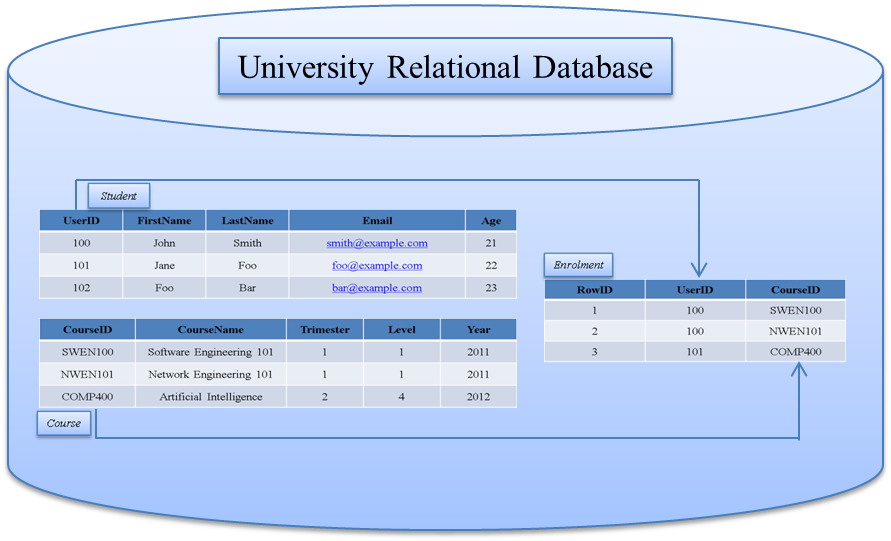
\includegraphics[width=.8\textwidth]{./figure/Example/Relational-DB.png}
	\caption{University example as a Relational database}\label{f:RDB}
\end{figure}

This shows how the University database example is deployed as a \ac{RDB}.  When
data in the University example is modelled using the column-oriented key-value
data model,   the way it is stored is different.
Although key-value \acp{DBMS} are schema-less,   column-oriented key-value
\acp{DBMS} are not entirely schema-less and hold some information about the
databases as metadata , as seen in Cassandra~\citep{datastaxDataModel}.
Such \acp{DBMS} allow applications to model the way data is organised in a
traditional \ac{RDBMS}, whilst bringing more flexibility by denormalising data
and imposing no rigid structures or schema
requirements~\citep{cassandra,BOOK,datastaxDataModel}.
Therefore,   it allows applications to add data in the way they want and change
their schema (if needed),   without adhering to a rigid schema unlike the
traditional \acp{RDBMS}.

The building blocks of column-oriented key-value \acp{DBMS} are the columns,  
the Super Columns,   the Column Family and the Key Space.  Using the
University example,   these terminologies are explained below. 
Appropriate analogies are drawn with the \ac{RDB} University,   as
seen in Figure~\ref{f:RDB}, to better understand these column-oriented key-value
concepts.  Since the focus is on Cassandra's data model,   these concepts
are explained in the way Cassandra deploys them.  The example used
to describe the Cassandra data model adopts a simple and flexible schema that
allows some structure in the way data is stored. 

\begin{description}
\item[Columns:]  A column is the basic unit of data in this data model.  It is a
tuple containing a column name,   a value and a timestamp (Figure~\ref{f:column}). 

\begin{figure}[h]
	\centering
	%\includegraphics[width=5cm,   height=5cm]{. /figure/random. jpg}
	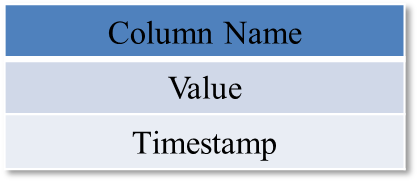
\includegraphics[width=.4\textwidth]{./figure/Example/Column.png}
	\caption{A column in Cassandra}\label{f:column}
\end{figure}

The column names are labels  and it is mandatory that a column has a name. 
Column names and values are stored as Bytes Type,   Long Type, Ascii Type,  
binary values Lexical UUID Type,   Time UUID Type or as UTF8 serialized
strings~\citep{BOOK,datastaxDataModel}.  Timstamps are used to store the time of
the latest update made to the column and are thus used for conflict resolutions.  The timestamp values are commonly stored as microseconds,   but could be in any format that the
application chooses.  However,   timestamp formats have to be consistent across
the database so that is the same format across all columns.

Cassandra allows indexes to be created on column names.  These are called
Secondary indexes and are of type \texttt{Keys} in Cassandra.  When such
secondary indexes are used,   efficient queries can be specified using equality
predicates,   and can be made on ranges of columns too.  The latter ones are
called range queries.

A column name can be considered analogous to a column in a table in any
traditional \ac{RDBMS}.  To illustrate this analogy,
Figures~\ref{f:column-FirstName} and~\ref{f:RDB-User} show the differences
between the representation of values in \texttt{Student} in Cassandra and in an
\ac{RDBMS}.
It can be seen from these figures that a column in the column-oriented key-value
data model is similar to a single value in a row of a relational table.  For
example,   the data '\texttt{John}' in the relational table \texttt{Student} can
be considered equivalent to a single column in Cassandra.

\begin{figure}[H]
	\newcommand{\W}{.2\textwidth}
	\centering
	%\includegraphics[width=5cm,   height=5cm]{. /figure/random. jpg}
	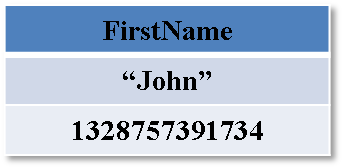
\includegraphics[width=\W]{./figure/Example/Column_FirstName.png}
	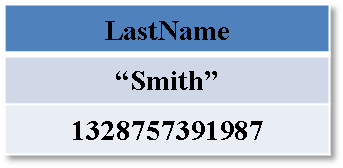
\includegraphics[width=\W]{./figure/Example/Column_LastName.png}
	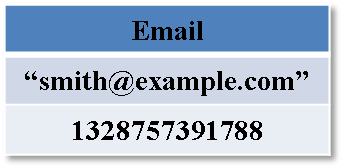
\includegraphics[width=\W]{./figure/Example/Column_Email.png}
	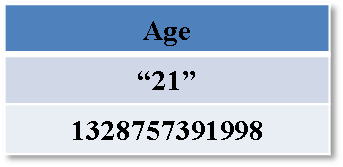
\includegraphics[width=\W]{./figure/Example/Column_Age.png}
	\caption{Columns in Cassandra}\label{f:column-FirstName}
\end{figure}

\begin{figure}[h]
	\centering
	%\includegraphics[width=5cm,   height=5cm]{. /figure/random. jpg}
	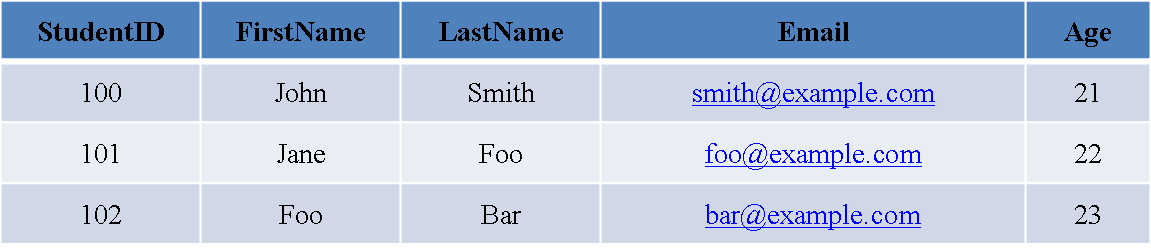
\includegraphics[width=.8\textwidth]{./figure/Example/RelationalTable_User.png}
	\caption{Relational Table - Student}\label{f:RDB-User}
\end{figure}

The JSON notation for  columns in Cassandra is shown in Figure~\ref{f:column-JSON}. 

\begin{figure}[H]
	\centering
	%\includegraphics[width=5cm,   height=5cm]{. /figure/random. jpg}
	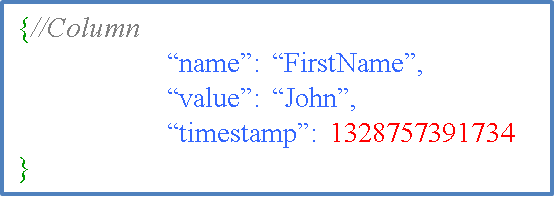
\includegraphics[width=.4\textwidth]{./figure/Example/Column_JSON.png}
	\caption{JSON notation for a column}\label{f:column-JSON}
\end{figure}
% 
% Alternatively,   applications can also use column names to store values.  This is
% possible since it is not required that columns always have values and
% since column names are byte arrays,   applications can store any kind of
% values in it. 

\item [SuperColumns:] A super column is a different kind of a column where the
values are an array of regular columns (Figure~\ref{f:supercolumn}).  It consists of a super
column name and an ordered map of columns.  The columns within the values of a
super column are grouped together using a common look-up value,   which is
commonly referred to as the \texttt{RowKey}.  In other words,   a super column is a
nested key-value pair of columns.  The outer key-value pair forms the super column while the inner
nested key-value pairs are the columns.  Unlike regular columns,   super columns do
not have timestamps for its key-value pairs.  

\begin{figure}[H]
	\centering
	%\includegraphics[width=5cm,   height=5cm]{. /figure/random. jpg}
	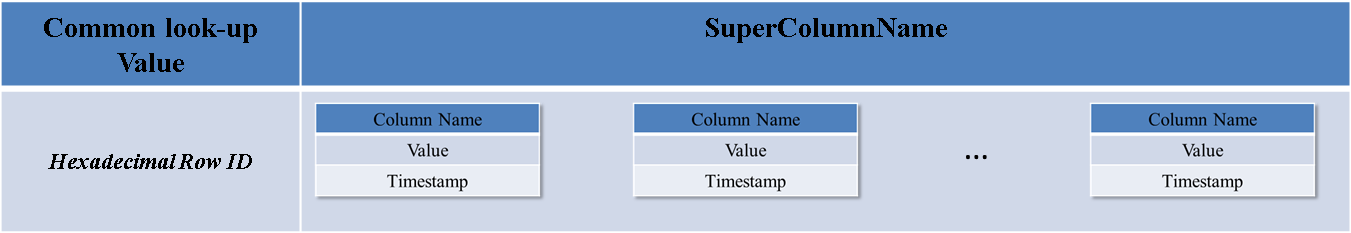
\includegraphics[width=.8\textwidth]{./figure/Example/SuperColumn.png}
	\caption{A Super Column }\label{f:supercolumn}
\end{figure}

A super column can be considered roughly similar to a whole record in a
relational table in an \ac{RDB}. For example,   the super column for a
student,   as seen in Figure~\ref{f:supercolumn-John},   is analogous to a single
record in the relational table \texttt{Student} (Figure~\ref{f:RDB-User}). 

\begin{figure}[H]
	\centering
	%\includegraphics[width=5cm,   height=5cm]{. /figure/random. jpg}
	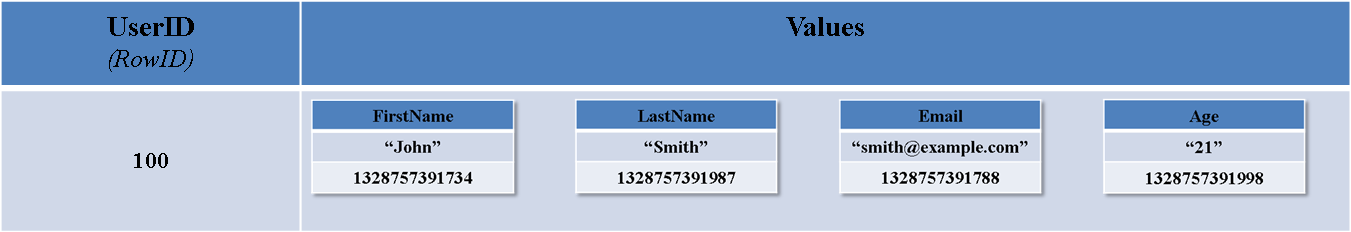
\includegraphics[width=.8\textwidth]{./figure/Example/SuperColumn_John.png}
	\caption{A Super Column for Student '\texttt{John}' in
	Cassandra}\label{f:supercolumn-John}
\end{figure}

The JSON notation for a super column is shown in Figure~\ref{f:supercolumn-JSON}. 

\begin{figure}[H]
	\centering
	%\includegraphics[width=5cm,   height=5cm]{. /figure/random. jpg}
	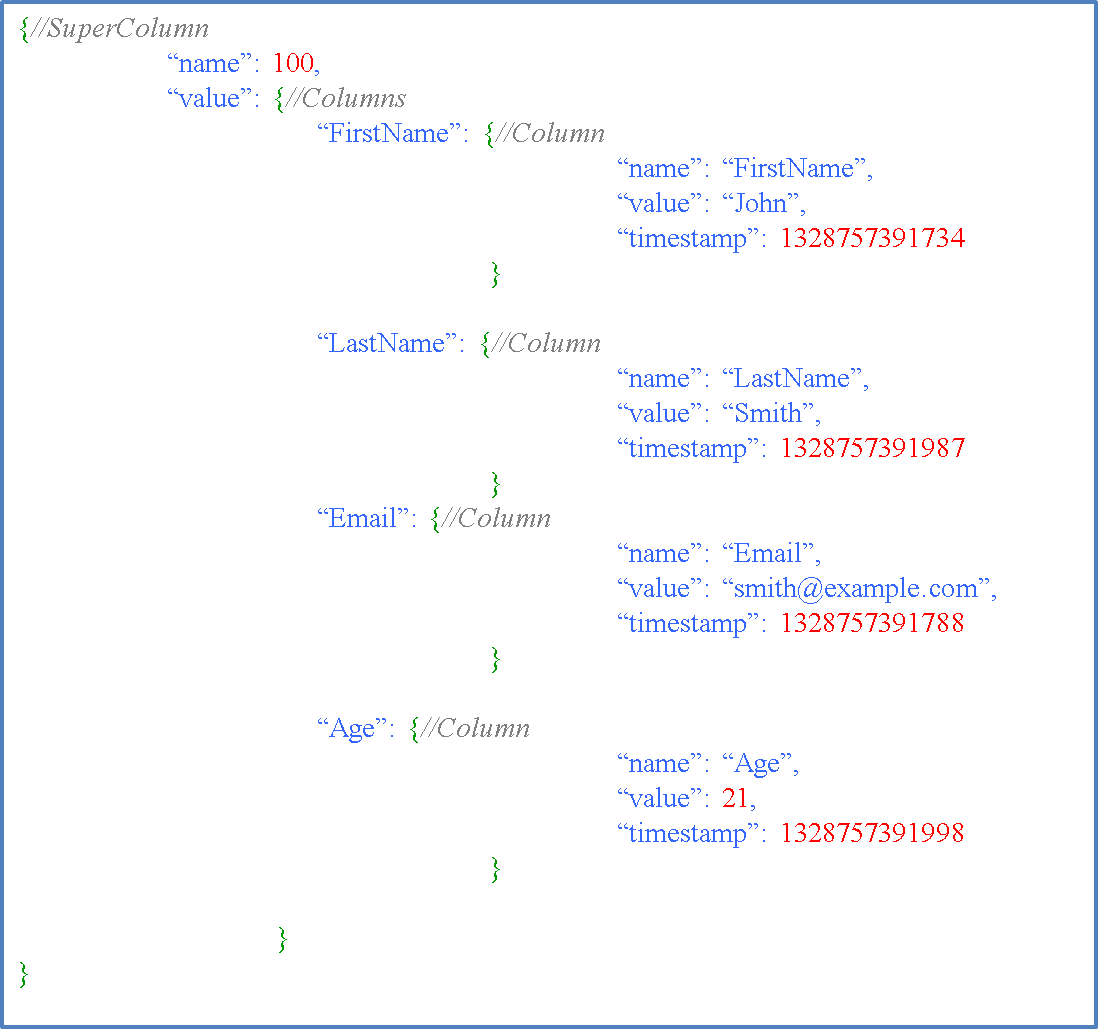
\includegraphics[width=.6\textwidth]{./figure/Example/JSON_SuperColumn_John.png}
	\caption{JSON notation for a super column}\label{f:supercolumn-JSON}
\end{figure}

\item [ColumnFamily:] A column family contains columns or super columns that are
grouped together using a unique row key.  It is a set of key-value
pairs,   where the key is the row key and the value is a map of column names
(Figure~\ref{f:columnfamily}).  The row key groups the columns together,   just as
in super columns. 

\begin{figure}[H]
	\centering
	%\includegraphics[width=5cm,   height=5cm]{. /figure/random. jpg}
	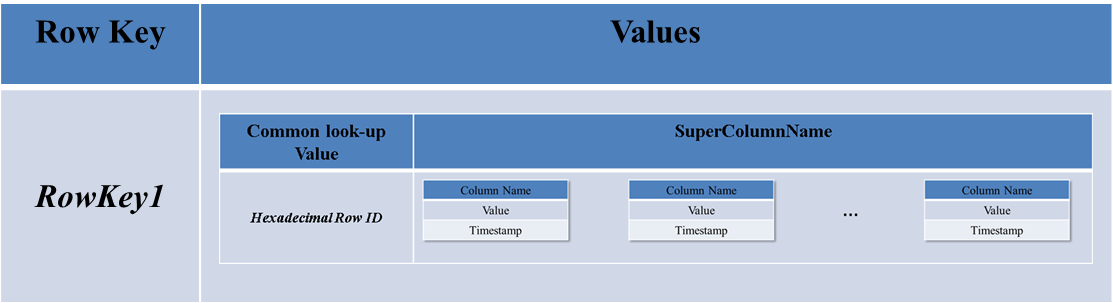
\includegraphics[width=.8\textwidth]{./figure/Example/ColumnFamily.png}
	\caption{Column Family in Cassandra}\label{f:columnfamily}
\end{figure}

Applications can define column families and metadata about the columns. 
It is commonly practised to have columns that are related or accessed
together to be grouped in the same column family.  Column families require that
some attributes are always defined,   like name,   column type and others.  It
also has optional attributes that can be defined if the application requires so.
 Some of the optional attributes are number of keys cached,   comments,   read
repairs,   column metadata among others.

Column families can have rows %to have relatively a definite number of columns. 
that are identified by their unique row keys.  This is similar to a table,   as
seen for table \texttt{Student} in Figure~\ref{f:RDB-User},   where every row in
the table has the same number of columns and primary keys are used to identify a
row.  An example of a column family is shown in Figure~\ref{f:columnfamilyUSER}.
Unlike relational tables in an \ac{RDB},   column families do not require all
the rows to define the same number of columns~\citep{datastaxDataModel,BOOK}.

\begin{figure}[H]
	\centering
	%\includegraphics[width=5cm,   height=5cm]{. /figure/random. jpg}
	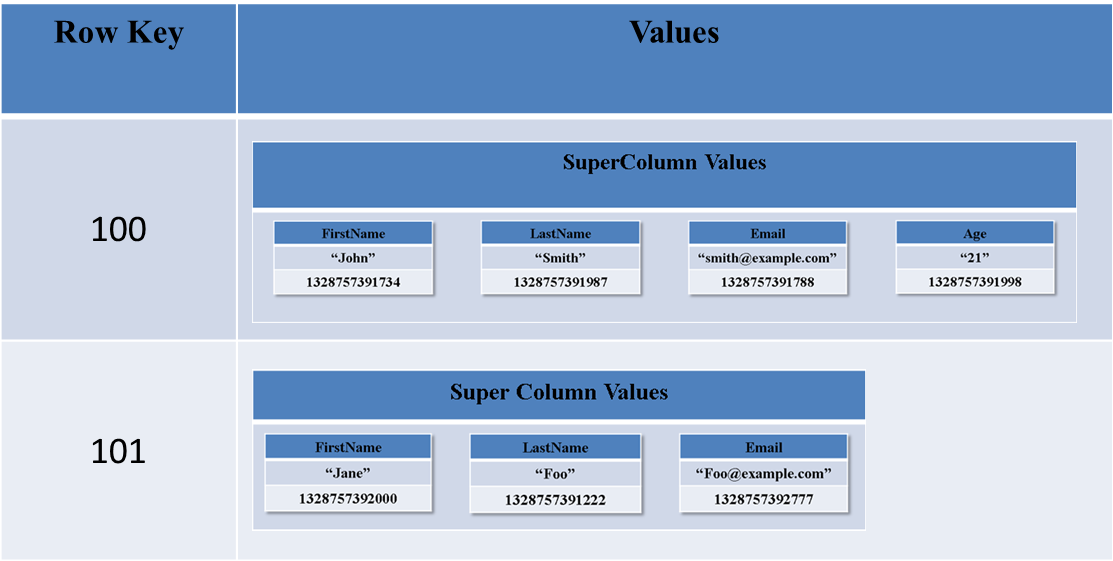
\includegraphics[width=.8\textwidth]{./figure/Example/ColumnFamily-User-DiffColumns.png}
	\caption{Column Family \texttt{User} in Cassandra}\label{f:columnfamilyUSER}
\end{figure}

The JSON notation for a single row of a column family in Cassandra is
shown in Figure~\ref{f:columnfamilyJSON} 

\begin{figure}[H]
	\centering
	%\includegraphics[width=5cm,   height=5cm]{. /figure/random. jpg}
	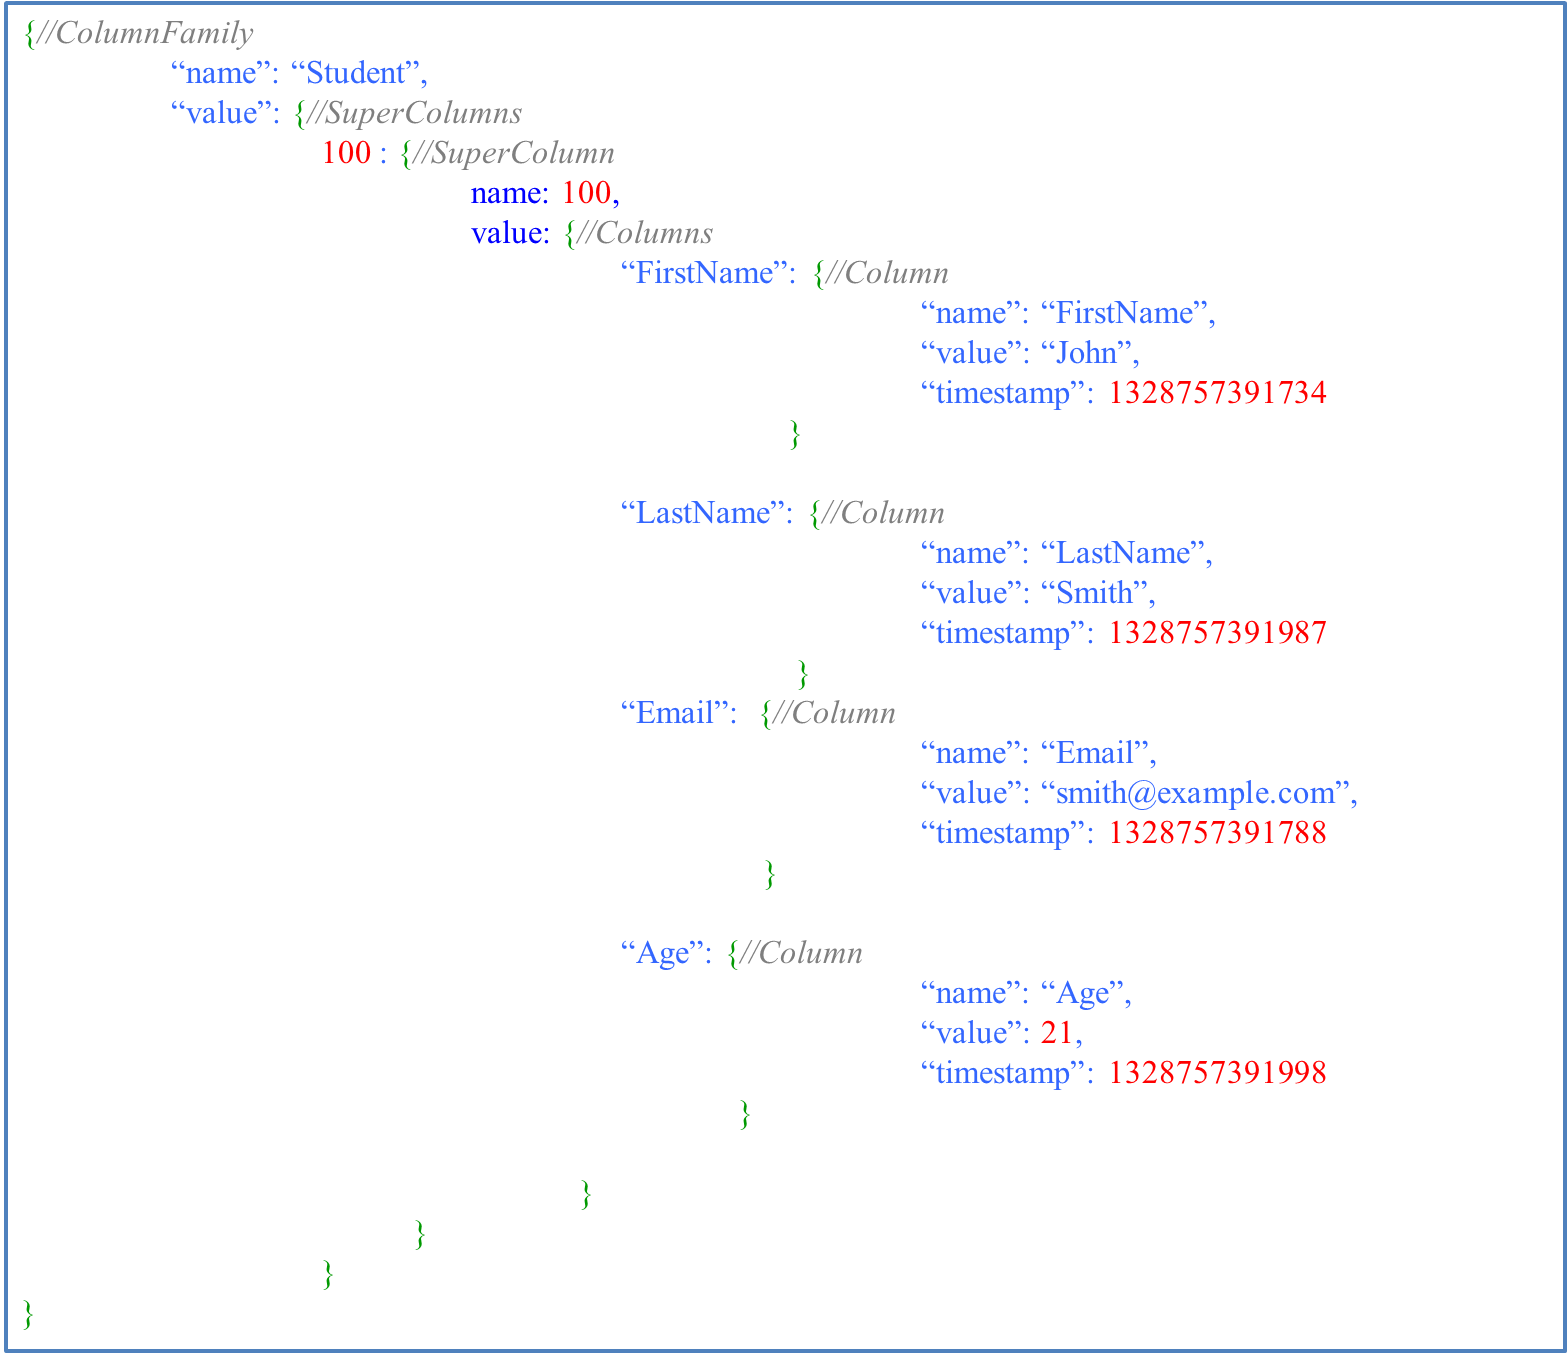
\includegraphics[width=.7\textwidth]{./figure/Example/JSON_ColumnFamily_1row.png}
	\caption{JSON notation for a column family in
	Cassandra}\label{f:columnfamilyJSON}
\end{figure}

\item [KeySpace:] A keyspace is a container to hold the data that the
application uses.  Keyspaces have one or more column families,   although it is not strictly
required that a keyspace should always have column families.  Any relationships
existing between column families in a keyspace are not preserved. 

A keyspace can be considered similar to a database in traditional relational
databases,   without any relationships.  An example of the keyspace
University is shown in Figure~\ref{f:keyspace}. 

Keyspaces require that some attributes are defined,   like a user defined name,  
replication strategy and others.  Some optional elements that can be defined are
the details of the column families in the keyspace and other options
for replication of data. 
\end{description}

%\newpage

\begin{figure}[h]
	\centering
	%\includegraphics[width=5cm,   height=5cm]{. /figure/random. jpg}
	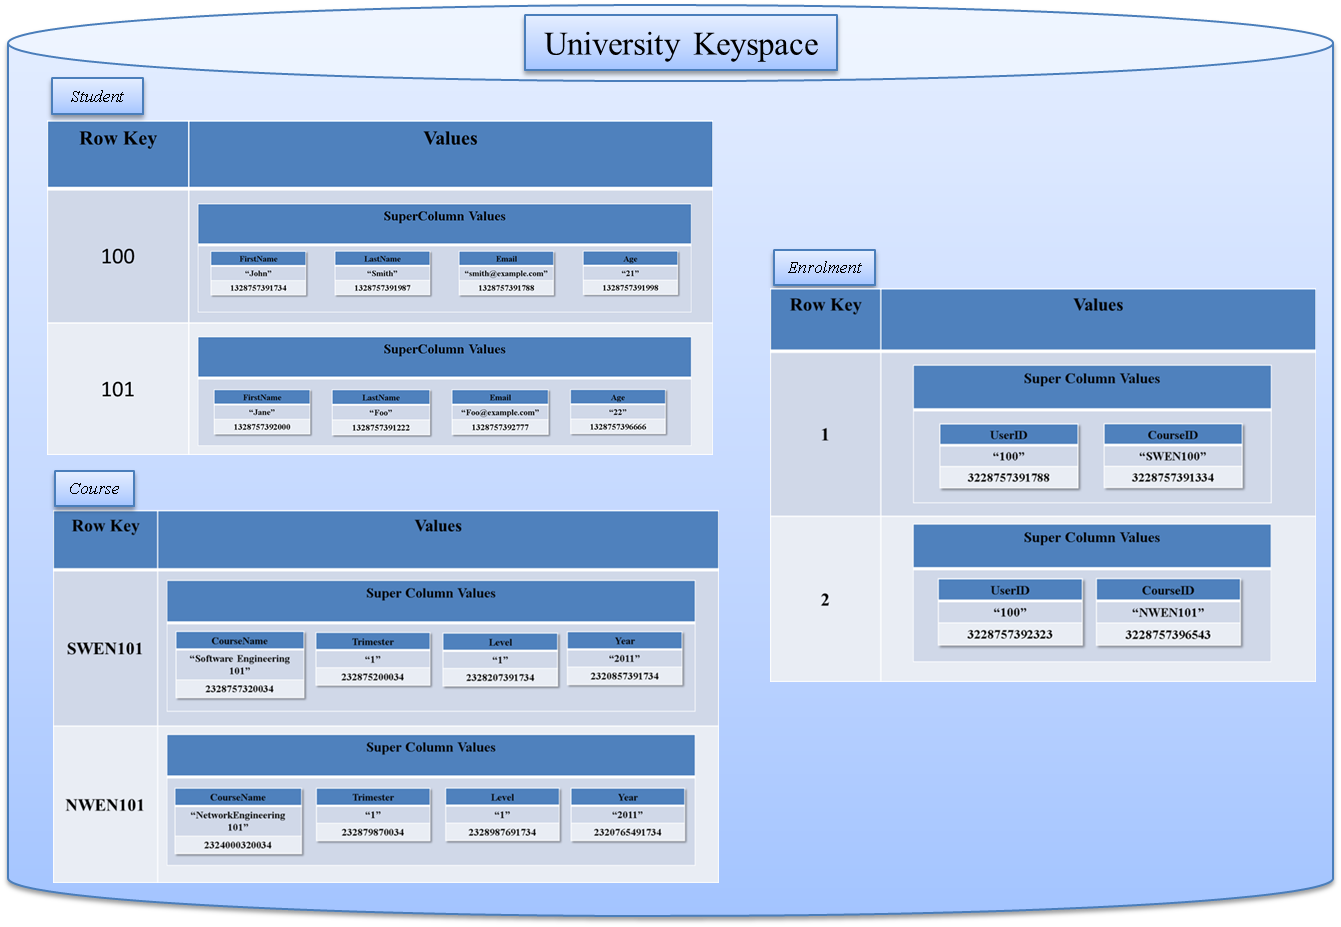
\includegraphics[width=.9\textwidth]{./figure/Example/KEYSPACE.png}
	\caption{A keyspace in
	Cassandra}\label{f:keyspace}
\end{figure}

As previously mentioned,  cloud \ac{NoSQL}
\acp{DBMS} are generally specialised to address specific problems like
partition-tolerance,  high availability among others and for this some
trade-off are made when these are developed.
Some of the challenges and problems present in such \acp{DBMS} are discussed in the following section.


%ब
\section{Challenges in the Key-Value Data Model}\label{s:challenges-key-value}
Fundamentally,   the key-value data model is different from the relational model
in many ways.  While the relational data model aims at giving data a structure,  
providing data integrity,   the key-value data model just
store data as \acp{blob} or string values and generally do not maintain
relationships between data.  In the column-oriented key-value model,   the
key-value association and the grouping of columns in column families can be
considered as the minimum relationship that is maintained.

According to~\citet{Bell},   data dependencies
are the most common types of semantic constraints in relational databases and these
determine the database design.  Data dependencies are the various relationships
that may exist between data entities in a database.  For example,   in the
University database,   a student can enrol into more than one course and this
means that there is a many-to-many relationship between \texttt{Student} and
\texttt{Course} since   one course can have many students enrolled in it.

As seen in Section~\ref{s:key-value-data-model},   the \texttt{Enrolment} table
contains the \texttt{StudentID} and the \texttt{CourseID} as foreign keys, thus
showing the dependency or relationship between students and courses
(Figure~\ref{f:RDB}).
In the \texttt{University} \ac{RDB} any attempt to delete a course from the
\texttt{Course} table,   is prevented by a constraint,   unless the dependency
itself is removed first.  In \acp{RDBMS} ,   this constraint is referential
integrity,   which ensures that references between data entities are valid,
consistent and intact~\citep{blaha,date}.
Normalisation,   as well as modelling real world data and relationships enforce
such dependencies in the schema and this causes integrity constraints like
referential integrity constraints,   to be imposed on data entities.

If such constraints are not imposed,   there could arise many dangling
dependencies in the database.  For instance,   consider the case of foreign key
references between \texttt{Course} and \texttt{Enrolment} in the  University
database.  If a course is deleted from the \texttt{Course} table without
removing its dependencies in \texttt{Enrolment},   the latter will contain
active references to the deleted course.  Another example of a dangling
reference occurs during insertion of data,   where a new student is entered in
the \texttt{Enrolment} table,   with a \texttt{CourseID},   that does not exist
in the \texttt{Course} table (i. e. ,   wrong \texttt{CourseID}).  A dangling
reference occurs because this inserted student refers to a nonexistent course.
Such problems cause inconsistent data to be stored in databases and violate data
integrity.  In order to ensure that users get consistent and valid information,
applications  have to implement mechanisms to check or prevent dangling
references.  However, if referential integrity constraints are applied as in an
\ac{RDB},   operations on data that  adversely affects referential integrity  
will not permitted.

As previously mentioned,   \ac{NoSQL} database systems do not normalise data and
nor are any relationships maintained.  However, relationships or dependencies
between data are common when real world data is stored in databases.  For
example,   in the real world,   a course could be taught by more than one
lecturer or a student with an Art major is restricted entry into Chemistry
courses etc.  These relationships and constraints have to be preserved upon
storage in cloud \ac{NoSQL} database systems too.  As mentioned in
Section~\ref{s:cloud-databases},   cloud databases,   whether relational or
\ac{NoSQL},   have to replicate data across several machines and need to be
scalable to match the needs of the users.  The replicated and distributed nature
makes maintaining data dependencies complex and unfeasible in terms of speed and
efficiency.  In cloud \ac{NoSQL} databases,   this effectively means that the
relationship between \texttt{Enrolment}, \texttt{Student} and \texttt{Course}
tables will not be strictly enforced and deleting a course in cloud \ac{NoSQL}
databases is allowed because of the absence of constraints.  As mentioned
before,   this means that students could still be enrolled in deleted courses,  
since there are no constraints to prevent such deletions or changes in cloud
\ac{NoSQL} databases.

Commonly,   developers impose such constraints and reference checks on
\ac{NoSQL} data at the application side.  Another way to implement such checks
is to give these constraints at the persistence layer of the application server.
 Both these ways  eventually have to handle all the processing and managing
of these constraint checks for all the widely spread data in \ac{NoSQL}
databases. However,   this could mean immense workload on the application or the
application server,   especially if the data volume is large in the \ac{NoSQL}
database or if it is has many replicas that have to be checked as well for the
constraints.


This is a serious problem when data is interconnected and dependant on other
data entities as is commonly the case.  For example,   consider a banking
application that uses cloud \ac{NoSQL} \acp{DBMS} where its data is
interconnected and spread across several nodes.  Any debit or credit
transactions made to a users account will have to be replicated across all the
nodes and correctly persisted.  Many constraints will exist for transfer of
funds between user accounts and such constraints need to be validated correctly.
 If a user has multiple accounts,   the relationship between the accounts have
to be maintained as well. Moreover, update operations may not be correctly
reflected across all the nodes of the database due to eventual consistency, 
 which is discussed in Section~\ref{s:Background-Cassandra}.
However, in spite of eventual consistency,   such constraints must be
correctly handled and recorded. When such constraints are not validated
correctly,   it leads to incorrect account balances and wrong updates in the
user accounts.  On the other hand,   when such applications use an \ac{RDBMS},  
referential integrity constraints are imposed to maintain the relationships
between the accounts where such constraints are defined when tables are created
and validations are triggered whenever any operations are performed on the data.

Although such problems mostly affect most cloud \ac{NoSQL} \ac{DBMS} users,   it
can be different for different users.  For example, a banking system as
mentioned above could be gravely affected because of dangling references while
in a simple game application such problems could be trivial.
% Addressing these challenges, implies to introduce referential integrity
% constraints in cloud \ac{NoSQL} database systems.
Motivated by such problems of data dependencies, this thesis studies the
existing modelling of data dependencies in cloud \ac{NoSQL} \acp{DBMS} and
contributes by proposing four solutions to effectively maintain and validate
referential integrity.
% while also not limiting the benefits of  \ac{NoSQL} \acp{DBMS}.
% In order to maintain referential  integrity in a database system, some rules
% and validations are performed when operations are executed on data items
% within a database.
The following section describes referential integrity and the rules that have to
be imposed within a database system to validate referential integrity.


%ब
\section{Referential Integrity in Key-Value
Model}\label{s:referential-integrity} 

Referential integrity is a fundamental property of data within databases,  
which ensures that data dependencies between tables are maintained correctly in
the database~\citep{blaha,date,Navathe,george}.  These dependencies
could be a part of the business rule and need to be enforced for proper data integrity.  Users define
conditions or rules on the tables in a database so that data integrity is
ensured at all times.  These conditions are called integrity constraints and
need to be mandatorily satisfied at all times in order to ensure that users or
applications do not enter incorrect or inconsistent data into the databases.

The Referential Integrity Constraint is just one amongst other constraints,  
and generally in \acp{RDBMS},   these constraints ensure that the value of
foreign keys in a table matches the values of primary keys in another table. 
The table containing the foreign key is the referencing table (or child table),
while the table with the primary or unique key is the referenced table (or
parent table).
For example,   in the University database,   \texttt{Enrolment} is the
referencing table while \texttt{Student} and \texttt{Course} are the referenced
tables.  Foreign keys are also known as the referencing key and
the primary keys as the referenced keys. 

It has been defined by many researchers that referential integrity is enforced
by the combination of a primary (or unique) key and a foreign key,   and that
every foreign key has to match the primary
key~\citep{blaha,Navathe,george,pathivada}.
In the University example,   every foreign key in the \texttt{Enrolment} table must
match one of the primary keys in the \texttt{Student} and \texttt{Course}
tables.
Hence,   if any foreign key refers to a non-existing primary key,   the
referential integrity constraint is violated.   For example,   if
'\texttt{StudID100}' is a foreign key for a student in the \texttt{Enrolment}
table,   but '\texttt{StudID100}' does not exist as a primary key in the
\texttt{Student} table,   then it is a violation of referential integrity.
 
Referential integrity constraints also describe the data manipulation that is
allowed on the referenced values.  Some of the widely associated rules are:

	\begin{itemize}
	
		\item \texttt{Restrict} or \texttt{No delete}: which prevents any update or
		deletion of data that has references. 
		
		\item \texttt{Set to NULL}: which sets all foreign keys to NULL values,   on
		updating or deleting the referenced key. 
		
		\item \texttt{Set to Default}: which sets all the foreign
		keys to a default value,   on updating or deleting the referenced key. 
		
		\item \texttt{Cascade}: which updates or deletes all the
		associated dependant values accordingly,   when the referenced data is updated or
		deleted. 
		
		\item \texttt{No Action}: which performs checks only at the end of a
		statement and is similar to \texttt{Restrict}
		
	\end{itemize}

Existing \acp{DBMS} may not always support all of the above rules.  Some \acp{DBMS} may
have the \texttt{Cascade} rule by default like Oracle,   while some may have the
\texttt{Restrict} rule by default.  

Generally,   in \acp{RDBMS} the database manager enforces a set of rules to
prevent any data operation,   like insert,   update or delete,   to change data
in such a way that referential integrity is not violated as seen in
Figure~\ref{f:RI}. 

	\begin{figure}[H]
		\centering
		%\includegraphics[width=5cm,   height=5cm]{. /figure/random. jpg}
		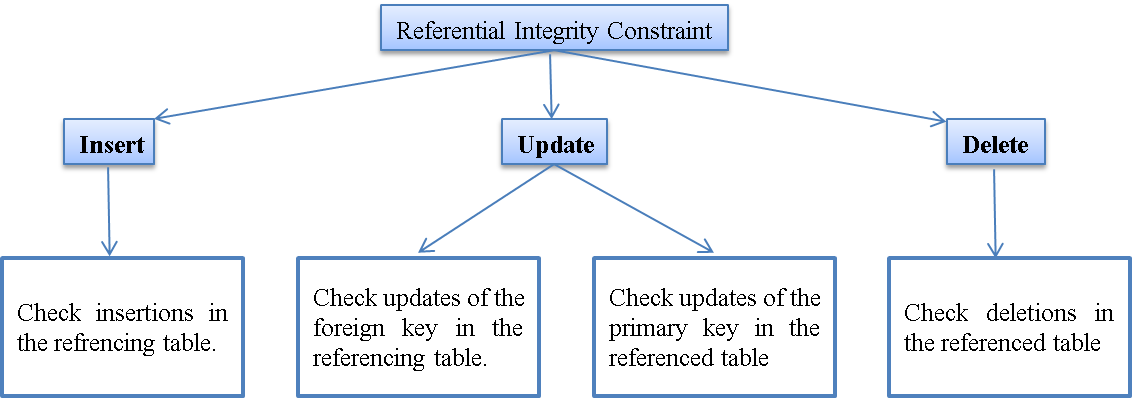
\includegraphics[width=.8\textwidth]{./figure/Example/RI-Figure.png}
		\caption{Referential Integrity Rules}\label{f:RI}
	\end{figure}

\todo{Fix this paragraph}
Referential integrity constraints have been a relational feature in traditional
\acp{RDBMS} and are imposed due to the way the \acp{RDBMS} enforce
normalisation.
In order to improve the data dependency in cloud \ac{NoSQL} \acp{DBMS},   this
thesis proposes solutions that implement referential integrity constraints using
different approaches. These solutions are
deployed and evaluated using Apache Cassandra, a column-oriented key-value cloud
Database Management System (DBMS). The following section gives an overview of
Cassandra and discusses some of its key architectural concepts.

% These rules are explained below:

% 	\begin{itemize}
\subsection{Insert rule}
		An insert operation triggers a referential integrity
		validation when data is being inserted into a referencing table,   i. e. ,   the
		child table.  In such an event,   prior to entering the values in the
		referencing table,   it is checked if the foreign keys exist in the referenced
		table.  For example,   in the University \ac{RDB},   when a row is inserted in
		the \texttt{Enrolment} table with foreign key values for \texttt{StudentID} and
		\texttt{CourseID},   a check is triggered to verify whether these foreign keys
		exist in the \texttt{Course} and \texttt{Student} tables as primary keys.  If
		the foreign keys do not exist in the referenced tables,   then the insert
		operation is not allowed.
		
\subsection{Update rule}
 When data is updated either in the referencing table or the
		referenced table,   a referential integrity validation is needed.  When any
		primary key is updated in the referenced table, then it is verified whether this
		key is a foreign key in any of the referencing tables.  If a dependency is found
		to exist,   then the applicable data manipulation rule is checked.  For
		instance,   if it is a \texttt{Cascade} rule,   then the associated foreign keys
		in the referencing table are updated prior to updating the key in the referenced
		table.  In the University \ac{RDB}, if the primary key '\texttt{SWEN100}' for a
		course is updated to '\texttt{SWEN101}',   then all the records in
		\texttt{Enrolment} that have '\texttt{SWEN100}' as a foreign key have to be
		updated to '\texttt{SWEN101}', if it has a \texttt{Cascade} rule.
		
		When any foreign key is being updated in a referencing table,   then a
		referential integrity validation has to be performed.  It is ensured that the
		new updated value exists as a primary key in the referenced table.  For example,
		  in the \texttt{Enrolment} table,   if \texttt{CourseID} in a row is updated to
		a new value,   then it is verified that the new value is an existing primary key
		in the \texttt{Course} table.  If the new value does not exist,   the update is
		not allowed generally.
		
\subsection{Delete rule} A delete operation triggers a referential integrity
		validation when data is deleted from the referenced table.  When data that is
		marked for deletion is found to have dependencies in other referencing tables,  
		the data manipulation rule applicable for this operation has to be checked. 
		This means that if the rule allows \texttt{Cascade},   then the depending values
		in the referencing table have to be removed prior to deleting values from the
		referenced tables.  For example,   when a student record is deleted from the
		\texttt{Student} table,   a check is performed to see if the
		'\texttt{StudentID}' is a foreign key in any other table.  Therefore,  
		\texttt{Enrolment} is checked and when the '\texttt{StudentID}' is found
		as a foreign key,   the appropriate action is performed depending on the data
		manipulation rule.  If it is '\texttt{Cascade}',   the enrolment details for the
		'\texttt{StudentID}' are removed from \texttt{Enrolment} and then the student
		record is deleted from
		\texttt{Student}. 
	
% 	\end{itemize}


 



%ब
\section{Apache Cassandra} \label{s:Background-Cassandra}

Cassandra is a distributed data storage system initially developed by Facebook
for satisfying the needs of large web applications that handle large
volumes of data~\citep{BOOK}. 
Its development has been undertaken by Apache  and it is  currently used by
many large web applications and large organisations like Facebook,  Twitter, 
Cisco,  Digg,  Reddit, and others~\citep{datastaxB}. 

Cassandra is based on the column-oriented key-value data model and stores data
as columns,  super columns,  column families and keyspaces, all of which are
explained in Section~\ref{s:key-value-data-model}. Being a distributed
system, Cassandra can run on multiple machines 
% runs as a single Java process on each machine in a cluster.
and provides the option  to work across different machines and across
multiple data centers,  even if these  are geographically
distributed~\citep{BOOK}.
These machines  are configured to operate together and
run as a single cluster, where these
% the entire cluster behaves like a unified whole. and access to only
% one of the nodes is required to perform operations.
 machines form a ring of nodes~\citep{datastax,BOOK}. Such
nodes are connected to each other and each node is aware of all their peers in
the cluster (Figure~\ref{f:cassandra-cluster}).


\begin{figure}[h] \centering 
	% \includegraphics[width=5cm,    height=5cm]{.  /figure/random.  jpg}
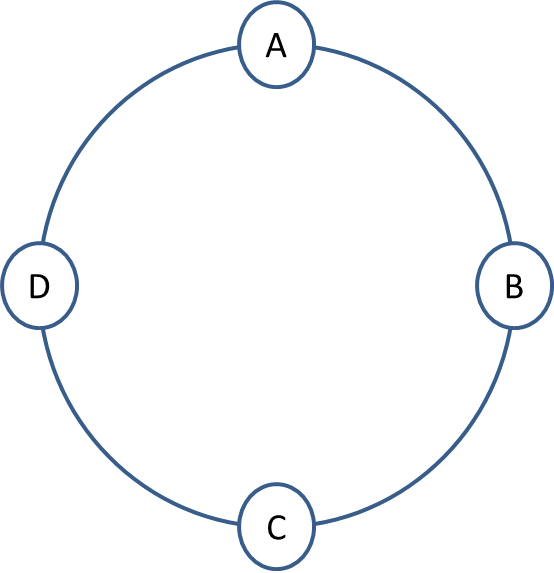
\includegraphics[width=.3\textwidth]{./figure/Background/CassandraCluster.png}
	\caption{A cluster of nodes in Cassandra}\label{f:cassandra-cluster}
\end{figure}

The nodes in a cluster communicate with each other to send their state
information at regular time intervals,  so that other nodes in the ring  know
their status~\citep{BOOK,cassandra}. Such communication
between the nodes support failure detection in Cassandra as when
% helps in failure detection in Cassandra since
 a node fails,  it stops responding to messages from other
active nodes and in this way the rest of the nodes  know of its inactive state.
% Cassandra is fault tolerant and able to perform operations despite node
% failures.
% Even when some parts of the cluster are inactive, Cassandra is fault tolerant
% and contiune performing its operations. 
In the event of a node failure,
operations sent to it are not lost since another active node ensures these are
performed~\citep{cassandra}.

In such a cluster,  every node applies the same architectural features
fundamental to Cassandra,  namely,  load balancing,  replicating
and partitioning data,  failure detection mechanisms, among others.  Some of the
key architectural concepts of Cassandra are explained next. 

% Distributed system are prone to conflicts as many users could be issuing
% requests on data items from any of the nodes.  Any distributed system should
% carefully consider conflict resolution and adopt design approaches which would
% resolve such conflicts efficiently.  Conflicts arise either at read or write
% operations. 
% The design approach should either make the system resolve such conflicts either
% during one of these operations,  deciding the system be either readable at all
% times or writable.  Cassandra optimises its performance by adopting the design
% approach of resolving conflicts during read operations,  making Cassandra always
% writable. 



\subsection{Architecture} \label{ss:Background-Cassandra-Archi}
Cassandra adopts many of its  architectural concepts from other popular
distributed key-value data storage systems on the cloud,  like Google's Bigtable
and Amazon's Dynamo~\citep{ycsb,Dynamo}.  Over time, these adopted concepts
evolved and developed new features,  some of which became specific to Cassandra's
architecture. Some of these  concepts are, peer-peer distribution model, data
partitioning, eventual consistency, among others. These  concepts gave Cassandra
  features such as elastic scalability,  fault tolerance, high availability and
high performance.
% Cassandra's architecture involves many sophisticated and complex theoretical
% as well as mathematical concepts,
% Following are some of the key architectural concepts of Cassandra.
% Discussing every concept is beyond the scope of this research.

\vfill

\subsubsection{Peer-Peer Distribution Model}
% Generally,  in traditional distributed
% \acp{DBMS},  nodes in a cluster are configured to have different
% responsibilities and roles where some or one of the nodes is a master and others
% are slaves.  Such a centralised configuration improves reading data,  as data can
% be read from any of the slave nodes,  but write requests are always sent to the
% master node.  This model thus puts a lot of additional load on the master and
% also is prone to failure if the single master node is offline.  However, 
Cassandra is a decentralised system  where all the nodes are considered equal
or identical (i.e.  nodes are peers) in sharing responsibilities and performing
operations,  without any  master or slave nodes~\citep{datastaxB,BOOK}. 
This model provides high data availability since failure
of a node does not affect the service of the cluster  because other
nodes carry out the same operation. 
% Moreover,  when new nodes are added to a cluster there is no additional task of
% delegating responsibilities or roles since all the nodes have the same
% responsibilites. 

% The nodes in a cluster communicate with each other to send their state
% information at regular time intervals,  so that other nodes in the ring can know
% their status (\todo{cite Cassandra paper}).  This helps in failure detection in
% Cassandra since if a node is not active it fails to send or respond to  messages
% from other active nodes and in this way the rest of the nodes  know of its
% inactive state.  In the event of a node failure,  another active node  performs
% the operations in order to ensure that  operations that were sent to a failed
% node are not lost (\todo{cite Cassandra papers}). 
% The recepient node  creates a small hint message with the information about
% the operation so that it can give the hint to the failed node once it is
% alive again and this feature is called hinted handoff. 

\subsubsection{Data Partitioning}
Cassandra partitions data between the nodes in a cluster  so that data items
from overloaded or failed nodes are assigned to other nodes or new nodes.  For
this,  Cassandra uses consistent hashing where data items are hashed on its key.
After hashing the key, the data items are assigned to the node whose
position in the ring is larger than the hashed value of the key~\citep{BOOK}.
% used by Amazon's Dynamo to partition data over the nodes. (\todo{DeCandia et
% al. (2007)}). 
% \begin{figure}[h] \centering %\includegraphics[width=5cm,    height=5cm]{. 
% /figure/random.  jpg}
% 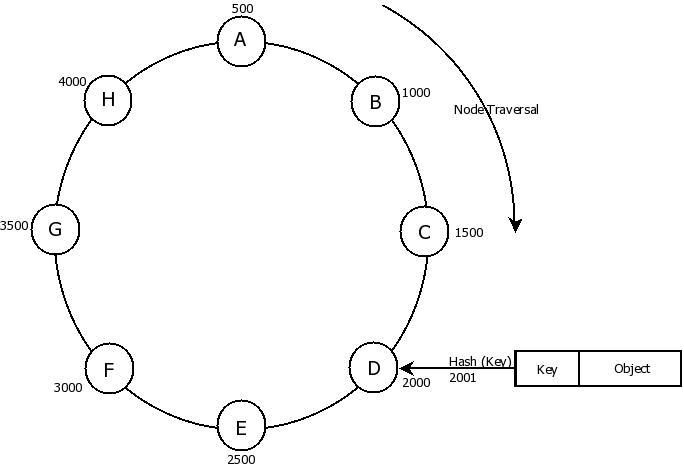
\includegraphics[width=. 6\textwidth]{. /figure/Cassandra/Consistent-hashing-Cassandra. png}
% \caption{Consistent hashing in Cassandra}\label{f:consistent hashing}
% \end{figure}
Data partitioning makes Cassandra elastically scalable since the load is
balanced and distributed in the cluster  irrespective of addition or removal of
nodes~\citep{BOOK,cassandra}. 
% Additionally,  in Cassandra better performing nodes are assigned multiple
% points in the ring,  making them virtual nodes and these nodes are assigned
% workloads from failed nodes or overloaded nodes. 

\subsubsection{Replication strategy} In order to ensure high data availability
irrespective of failures,  Cassandra uses a replication strategy where every
data item is replicated across a number of nodes.  Applications can set the
level of replication to suit its requirements,  that is, the replication factor
is set to the number of nodes on which the application wants to create
replicas~\citep{BOOK,cassandra}.  The
replication factor tells the cluster how many copies to create of a single data item.
Setting the replication factor to a large number will help in higher
consistency of data items,  but replicating data items to a large number of
nodes  can adversely affect the performance.

Once data items are partitioned and assigned to a node,  these are
replicated onto other nodes and a list of the nodes responsible for storing the
data items are maintained.  Thus, every node in the cluster knows which nodes
are responsible for a data item~\citep{BOOK,cassandra}.
Such a replication strategy makes data highly available  since data items can
be accessed from any node in a cluster regardless of node failures.  
% Since all
% the nodes  know which peer node is responsible for a data item,  
% routing requests to the correct nodes. 



\subsubsection{Eventual Consistency}
% As mentioned previously,  Cassandra opts for '\texttt{A}' and '\texttt{P}' of
% the CAP theorem and allows users to determine the level of consistency they
% prefer.  This consistency level tells the cluster how many replicas should
% acknowledge operations done on them,  for the replicas to be considered
% consistent and up to date.  Low consistency levels are considered better for
% performance as higher consistency levels involve more time since nodes have to
% wait to receive acknowledgements from more replicas.
% Letting the users decide the consistency level and replication factor means
% the tradeoff between consostency and performnace is detemined by the users.
In any strongly consistent  \acp{DBMS}, data items immediately reflect the new
values upon an insert or update operation. However, Cassandra uses the eventual
consistency model where replicas do not agree to the most recent value
immediately but will do so eventually. This is because the new values are
propagated to all the replicas in a cluster in an asynchronous
way~\citep{Tai,ycsb,henry,Vogel}.
% Eventual consistency provides Cassandra high scalability because any write or
% update operation  reaches all the replicas irrespective of the number of
% nodes in a cluster.
% Thus,  all replicas would be consistent eventually after a certain period of
% time, generally a small number of milliseconds \todo{cite book}.
% This is unlike strict consistency models  run on single nodes,  where a read
% operation always returns the most update values.
% In distributed systems like Cassandra,  several machines are used concurrently
% by many users leading to various conflicts,  which makes a weaker form of
% consistency like eventual consistency  ideal (\todo{cite BOOK and marked
% papers}).

 
\subsection{Write and Read Operations}
\label{ss:Background-Cassandra-Operations} 
In order to write data into Cassandra column families,  a write request is sent
to a random node in the cluster,  which acts as a proxy node and replicates the
data in the cluster~\citep{datastax,BOOK,cassandra}.
The number of nodes on which data is to be replicated can be changed to suit the
application requirements. Moreover, these nodes can be in the same data centre
and other data centres.

		

When a read request is issued to a node,  it acts as a proxy node and forwards
the request to all the other nodes in the cluster.
These nodes return their copy of the data item to the proxy node and the proxy
node  checks the versions of the replicas and sends the latest replica to the
user~\citep{datastaxRead}.   If the replicas received from a node are not
consistent with other replicas, a read repair is performed on the node
with the outdated replicas.  This means that the nodes with outdated replicas
are sent a write operation with the latest data.
Thus,  data consistency is maintained whenever conflicting versions of data
items are found.

When rows or columns are deleted in Cassandra, the  data within these rows or
columns is not removed immediately from the disk~\citep{datastax,BOOK}. Instead,
data is deleted after a time period that is configurable by applications. This
is called a tombstone delete in Cassandra, where the columns that are to
be deleted are only marked for deletion and empty values are written into such
columns.
Once the configured time period expires, the data is physically removed from the
disk. However, the row keys of the deleted columns continue to persist. Such a
tombstone delete is useful when a failed node is active again as this node can
update its replicas  correctly to show the deletions.




% Motivated by such problems of data dependencies,   this thesis studies the
% existing modelling of data dependencies in cloud \ac{NoSQL} database systems and
% aims to contribute by suggesting four solutions so that referential integrity
% is effectively maintained,   while also not limiting the benefits of not having
% a rigid schema in \ac{NoSQL} database systems.  Such a result would reduce the
% workload of the applications or the persistence layers of the application
% servers.  Additionally it would give users of \ac{NoSQL} database systems
% better consistency in data,   along with ensuring better data integrity even when
% it is widely replicated or spread on different data-centers. 


% These proposed solutions are deployed and analysed in Cassandra,  which is a
% column-oriented key-value \ac{DBMS}. To implement any solution it is necessary
% to understand the architecture and the key operations allowed in a \ac{DBMS}.
% For this purpose,  the architecture of Cassandra is discussed in the following section.



\section{Summary}



This chapter presented the background about the underlying concepts in cloud
computing and cloud databases.  It is clear that cloud computing is gaining
prevalence due to its many benefits like high data availability, cheap
storage, and others.  With an increase in the number of users
migrating to cloud computing,   cloud data storage is gaining prominence as well,  
for easy and simple data storage.  This has paved the way for the existence
of many different data models and databases on the cloud.  Amongst the many data
models, the key-value data model has been  most widely used  on the cloud
as it is more adapted to the cloud environment due to its support for
replication and scalability and other cloud related features (\todo{cite}). 



This chapter also discussed a few  architectural concepts of Cassandra that form
its foundation , providing it with BASE properties and many important features like
high data availability, failure management, fault tolerance and scalability
among others.  
The architectural concepts and operations of Cassandra are designed to
make it a highly available and scalable \ac{DBMS}.
Cassandra is used to implement the four solutions
designed to impose referential integrity validations in cloud \ac{NoSQL}
\acp{DBMS}.  The design of these solutions  and the approaches used to
implement such validations are explained in the following chapter. 


% The next chapter describes the four solutions proposed to enforce referential
% integrity constraints in cloud \ac{NoSQL} \acp{DBMS},   particularly in
% Cassandra which is based on the column-oriented key-value data model. 





